\documentclass[11pt]{amsart}
\usepackage{geometry}                % See geometry.pdf to learn the layout options. There are lots.
\geometry{letterpaper}                   % ... or a4paper or a5paper or ... 
%\geometry{landscape}                % Activate for for rotated page geometry
%\usepackage[parfill]{parskip}    % Activate to begin paragraphs with an empty line rather than an indent
\usepackage{graphicx}
\usepackage{amssymb}
\usepackage{epstopdf}
\usepackage{setspace} 
\usepackage{amsmath}
\usepackage[options]{algorithm2e}
\usepackage{float}


\DeclareGraphicsRule{.tif}{png}{.png}{`convert #1 `dirname #1`/`basename #1 .tif`.png}

\title{Brief Article}
\author{The Author}
%\date{}                                           % Activate to display a given date or no date
\usepackage{parskip}
\setlength{\parindent}{25pt}

\begin{document}
\begin{spacing}{1.0}
\maketitle
%\section{}
%\subsection{}

\section{Report}

In the previous chapter, we have seen that using a MFCC representation of utterances with regions of silence removed leads to a large improvement in accuracy, time and computational complexity in the performance of DTW algorithm augmented with a  euclidean metric.. From the experiments conducted  it is clear that  the main contributing factor behind the large time and computational complexity experienced by the base line DTW is the dimensionality of the time series sequences. The computational cost of a DTW algorithm is $(mn)$ where $m$ and $n$ denote the length of the two time series sequences currently being compared. Using longer sequences increases the size of the DTW cost matrix hence resulting into a greater number of computations.

The base-line DTW algorithm  is a domain independent  algorithm that  uses a similarity metric  to  compare  any two sequences through comparison of  their  global trends.  The algorithm  employes dynamic programming to search a space of mapping between the time axis of  the two respective sequences to determine the optimum alignment between them.  The only difference between MFCC-augmented DTW and baseline DTW is the feature extraction stage. In machine learning, feature extraction refers to the pre-processing stage that involves the extraction of new features from a set of raw attributes through a suitable functional mapping. The extraction phase of MFCC features  involves a segmentation of the time series followed by a functional mapping on the segmented windows. The  resultant sequence of  extracted feature vectors has a much smaller length compared to the length of the original sequence. Evident from the  experiments done in the previous chapters, the use mel-cepstrum features extracted on `cleaned' signals not only increases the accuracy of DTW but also reduces the time and computational cost through reduction of dimensionality of the original sequence.

 Time series sequences are embedded with local and global trends. Unsupervised methods using DTW  focus on  exploiting the information of either these trends for pattern extraction and mining. From the  work conducted by Xie and Wiltgen on  the time series datasets[], it  has been shown that using DTW equipped with features that incorporate  information of \textbf{both}  local trends and global shapes in the clustering /classification process greatly improves the performance of DTW . Unlike the MFCC, the features constructed from local and global trends are domain independent and thus can be applied to any time of data.  However, when working high-dimensional time-series data, the accuracy of the DTW algorithm using a window constraint suffers greatly even if it's equipped with domain dependent/independent features. Hence from a scientific point of view, it is of great interest to research methods to improve the DTW algorithm so it can constraint the time and computational complexity associated with high-dimensional data without degrading the accuracy by too much. In this chapter, I investigate an unsupervised methodology that:

\begin{itemize}
\item incorporates  information about local and global trends  in the feature extraction process
\item employs an adaptive DTW that tackles the issue of the large time and computational complexity by moving from working on  time series sequences to  sequences of segmented time-slices. To counter the tradeoff in the decrease  in accuracy, the algorithm is equipped with a kernel function(self-proposed) that is designed to measure the similarity of sub-sequences more accurately than standard euclidean metric by being invariant toward time-dilation and scale.   
\end{itemize}

\section {{Feature extraction}}


The fundamental problem of baseline DTW  is that the numerical value of a data point in a time series sequence is not a complete picture of the data point  in relation to the rest of the sequence. The context such as the position of the points in relation to their neighbours is ignored. To fix  this issue, an alternative  form of DTW know as \emph{Derivative} DTW is proposed but the fundamental problem with this DTW is that it  fails to detect significant common sub-patterns between two sequences(mainly global trends). Ideally we need to use features that contains information about the overall shapes of the sequences plus the local trend around the points. This allows the DTW to built a complete picture of the data point in relation to the rest of the sequence and hence achieve a better optimal alignment between the two sequences.

For feature extraction, the methodology that I have used  for this setup is based on Xie and Wiltgen's paper[].  Each point in the time series sequence is replaced by a 4 dimensional vector  where the first two features correspond to information regarding the local trends around a point and the last two features reflect the position of that point in the global shape of the sequence.

Definition of local feature given in [] is as follows:
\[ f_{\mbox{local}}(r_i)= (r_i-r_{i-1}, r_i-r_{i+1})\]



The  extraction of global features is constrained by two factors: the features that reflect information about  global trends and  the features must be in the same scaling order  as the local features. Being in the same scale allows them to  be combined with local features. In [] the authors used the following method to extract global features from the time series sequence:
\[ f_{\mbox{global}}(r_i)= (r_i -\sum_{k=1}^{i-1}\frac{r_k}{i-1} , r_i-\sum_{k=i+1}^M \frac{r_k}{M-i})\]

Note : The local and global features have no definition for the first and last points in a sequence.
\section{Adaption of DTW}
The feature extraction methodology discussed above maps the time series sequence to a time series sequence of vectors whose length  is $\|X_n\|-2. $   ( where $\|X_n\| $ denotes the  length of the original time series sequence).  The DTW augmented with these features will still suffer from large time and computational complexity if the dimensionality of the data is high. In the MFCC feature extraction process, the time series sequence is first segmented into series of frames  of length 20ms. Through appropriate functional mapping, each  frame is then mapped to a vector. Because the length of the resultant sequence of vectors is much smaller than the length of the original time series, the size of the  DTW cost matrix is reduced resulting in lower  time and computational cost associated with each comparison.

Similar to the MFCC extraction process, the time series of 4d vectors extracted in the feature extraction stage are segmented using windows  of width 5ms. The original time series is reduced to series of matrices  where the length of the new  series is 5 times smaller than before. Now if we adapt the cost function of DTW to work on series of matrices rather than series of vectors we can achieve a large improvement in the time and computational cost  associated in the testing phase without imposing a \textbf{window} constraint. 

The problem now can be shifted to finding  an appropriate kernel that can be used to compute the similarity between matrices composed of feature vectors. Ideally, we want a metric that takes into account the variation of speed and time when comparing two similar subsequences. We will want to compare the global and local properties associated with a point in one subsequence with the global and local properties of points at  different regions in the second sub-sequence illustrated by figure 2.  Using a euclidean metric in this scenario is inappropriate. The euclidean metric  in this context is identical to  linear time warping where the  two subsequences will be matched based on a linear match of the two temporal dimensions.  In our context, we need a kernel that computes the similarity between two sub-sequences by warping the time axis.

The motivation behind the kernel  that I propose for aiding  DTW to tackle  high-dimensional data comes from the polynomial kernel. \\
Let $x$ and $z$ be two dimensional vectors.
Consider the simple polynomial kernel of degree 2  :$k(x,z) = (x^{T}z)^2$ .  This kernel can expressed as :
\begin{eqnarray*}
k(x,z) &= &(x^{T}x')^2\\
&  =& (x_1z_1+x_2z_2)^2\\
&= & x_1^2z_1^2 + 2x_1z_1x_2z_2 + x_2^2z_2^2\\ 
&=& (x_1^2, �2x_1x_2, x_2^2)(z_1^2, �2z_1z_2, z_2^2)^{T}\\
&=& \phi(x)^{T}\phi(z)\\
\end{eqnarray*}\\
The 2nd order polynomial kernel is equivalent to a corresponding feature mapping $\phi$  that contains terms of order 2. Now, if we generalise this notion then $k(x,z) = (x^{T}z)^M$ contains all monomials of order M. If we imagine x and z to be two images, then the polynomial kernel represents a particular weighted sum of all possible products of M pixels in the first image with M pixels in the second image.\\
Using this as motivation I propose the following kernel:.
\[ k(x,z) = <\sum_{i=1}^{n}x_i, \sum_{j=1}^{n}z_j>\]
where $n$ denotes the length of the window and $x_i$  and $z_j$ represents the 4-dimensional features indexed by the points in two sub-sequences.\\
To motivate the reasoning behind the construction of this particular kernel lets consider the following signals:
\begin{figure}[H]
  \centering
   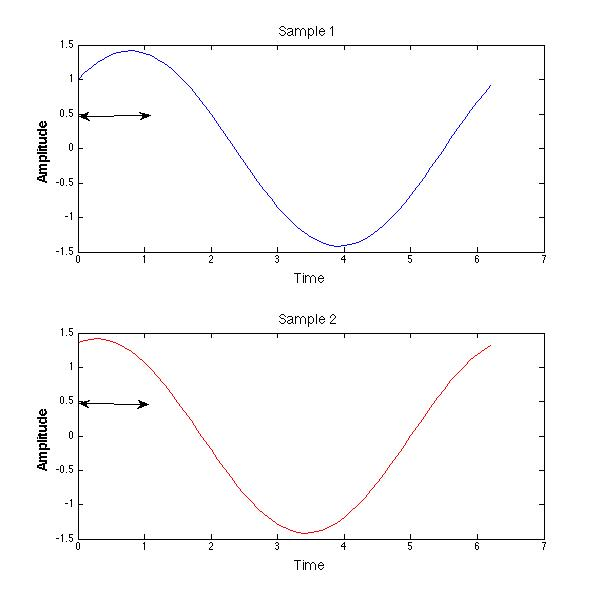
\includegraphics[scale=0.4]{Example1.jpg}
  \caption{Two signals separated by translation}
 \end{figure}
The signal denoted by the `red' color is a `slower' version of the signal denoted by the `blue' color . In the above example, if we are comparing the similarity  between the  time slices spanned by the arrows, an ideal kernel must be invariant to  the time offsets of the signals and thus should consider all possible pairings between the vectors in the subsequences. Intuitively speaking, the kernel must behave like a DTW algorithm..\\
\begin{figure}[h!]
  \centering
   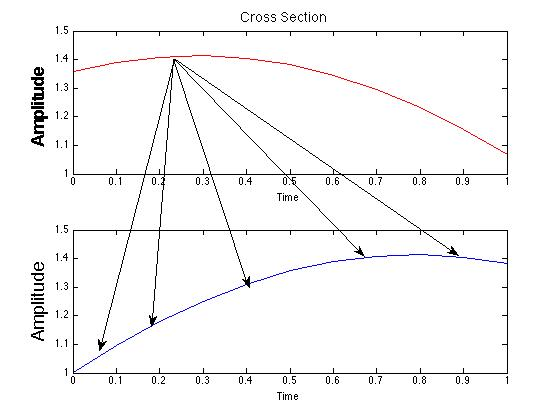
\includegraphics[scale=0.6]{Cross-section.jpg}
  \caption{Two identical subsequences varying in time }
  \end{figure}
 For time slices of width $n$, the kernel  metric  can be expanded and   expressed as :
\begin{eqnarray*}
k(x,z) &= &<\sum_{i=1}^{n}x_i, \sum_{j=1}^{n}z_i>\\
&  =& <(x_1+x_2+x_3+..),(z_1+z_2+z_3+..)>\\
&= & <x_1,z_1>+<x_1,z_2>+<x_1,z_2>...+<x_2,z_1>+<x_2,z_2> +<x_2,z_3>+......\\ 
\end{eqnarray*}
From above expression, we can see  that the proposed kernel corresponds to a sum of all possible dot products of pairs belonging to the set
$\{(x_iz_i) | x_i\in \mbox{seq1}, z_i \in \mbox{seq2}\}$. Similar to the polynomial kernel, the proposed kernel  allows us to match all possible pairs of vectors belonging to the two sub-sequences  given by the matrices.
It is easy to check that this proposed kernel is in fact a valid kernel:
\begin{itemize} \itemsep-2pt
\item K(x,z)= K(z,x) $\Rightarrow $the function is symmetric.
\item The kernel satisfies Mercer's theorem : K(x,z) =$\phi(x)^T\phi(x)$
where  the feature mapping corresponds to  a finite summation of vectors $\phi(y) = \sum_{i=1}^{n}y_i$. 
\end{itemize}
Augmenting the kernel to the DTW algorithm allows DTW to work on high-dimensional time sequences with using a window constraint. However the accuracy and computational cost of the DTW is now dependent on the size of the time slices used to segment the original sequences:
\begin{itemize} \itemsep-2pt
\item The accuracy of DTW increases as the width of the windows decrease. Using subsequence allows the similarity measure to be dominated by the dot products of points whose local and global features are most alike. However using smaller windows achieve lesser dimensionality reduction. Thus the time and computational complexity suffers.
\end{itemize}
To use this kernel as an  appropriate cost function in the DTW algorithm, we need a functional mapping that:
\begin{enumerate} \itemsep-2pt
\item  constraints the codomain to be in the range from 0 to $\infty$.
\item    ensures larger values given by the function signify great degree of dissimilarity and smaller values  signify a high degree of similitude.
\end{enumerate}
An ideal cost function that make use of dot product sis the \emph{arc-cosine}. Hence I embedded the kernel function in the cosine distance: 
\[ \theta = \frac{ <X,Z>}{|X||Z|} \]
where $X = \sum_{i=1}^{n}x_i$ and $Z =\sum_{j=1}^{n}z_i$

A formal outline of the algorithm is as follows:

\begin{algorithm}[H]
 \SetAlgoLined
 \KwData{seq1, seq2}
 \KwResult{cost }
 Segment the sequences using a window of size n\\
 seq\_1$\leftarrow$segment(seq1,n)\\
 seq\_2$\leftarrow$segment(seq2,n)\\
 
 Augment a matrix of 0 vectors to the front  seq1` and seq2`   \\ 
 Initialise the DTW cost matrix\\
 \For{i=1: to length(seq\_1) }{DTW(i,0) = $\infty$}\EndFor
 \For{i=1 to length(seq\_2)} { DTW(0,i) = $\infty$}
 \EndFor 
 \For{i=2 to length(seq\_1)}  {
 \For{j=2 to length(seq\_2)} {
 DTW(i,j) = $\theta = \frac{ <X,Z>}{|X||Z|}  + min\{ DTW(i-1,j)+DTW(i,j-1)+DTW(i-1,j-1)\\
 where  $X = \sum_{i=1}^{n}x_i$ and $Z =\sum_{j=1}^{n}z_i$ }
 \EndFor}
\EndFor
 cost = DTW(length(seq\_1),length(seq\_2))
  \caption{Adapted DTW algorithm}
\end{algorithm}
\newpage

\section{Experimental results}
The main aim behind the design  of the proposed DTW(discussed in the last section) is to improve the accuracy of the DTW algorithm while restricting time and computational cost to  a minimum
when applied to high-dimensional time-series data. I have tested the algorithm on the test data set that I have constructed using TIDIGITS test corpus and compared the performances against the methodologies that I have investigated so far:
 
\begin{itemize}
\item Methodology 1
\begin{itemize}
\item Apply feature selection process to remove segments of silence and down sample the remaining segment to improve the quality.
\item  Apply value-based DTW(which we denote as baseline) using the most constrained window size  and a euclidean metric.
\end{itemize}

\item Methodology 2
\begin{itemize}
\item Apply feature selection process to remove segment of utterance and down sample the remaining segment to improve the quality.
\item Apply  the feature extraction process discussed in [] to extract local and global features.
 \item Apply DTW using the most constrained window size  and a euclidean metric.
 \end{itemize}

\item Methodology 3
\begin{itemize}
 \item Apply no feature selection
 \item Perform feature extraction by extracting MFCC features
 \item Apply DTW using the most constrained window size and a euclidean metric.
 \end{itemize}
 
 \item  Methodology 4
 \begin{itemize}
 \item Apply feature selection process that only removes  segments of  silence 
 \item Extract MFCC features
 \item Apply DTW augmented with the euclidean metric.
 \end{itemize}
 \end{itemize}
I raw this algorithm on 3 different sets of data sets:
\begin{itemize}
\item The test and training sets that I have created from the Tidigits samples
\item To data sets  from the UCR time-series testbed:
\begin{itemize}
\item  The ECG torso datasets
\item The Inline Skating datasets.
\end{itemize}
\end{itemize}
\begin{figure}[h!]
  \centering
   
     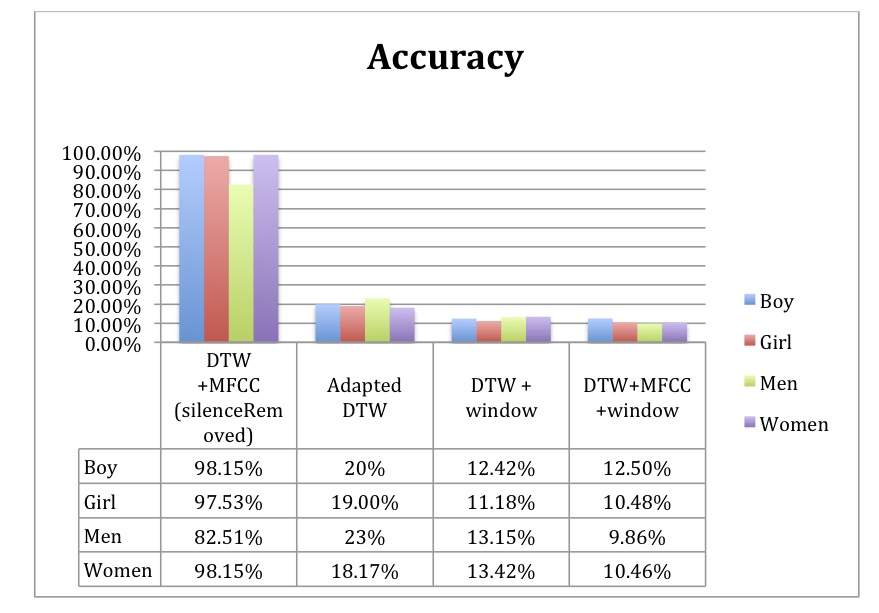
\includegraphics[scale=0.8]{Accuracy.jpg}
  \caption{Accuracy}
  
\end{figure}
\end{spacing}
\begin{figure}[h!]
  \centering
   
     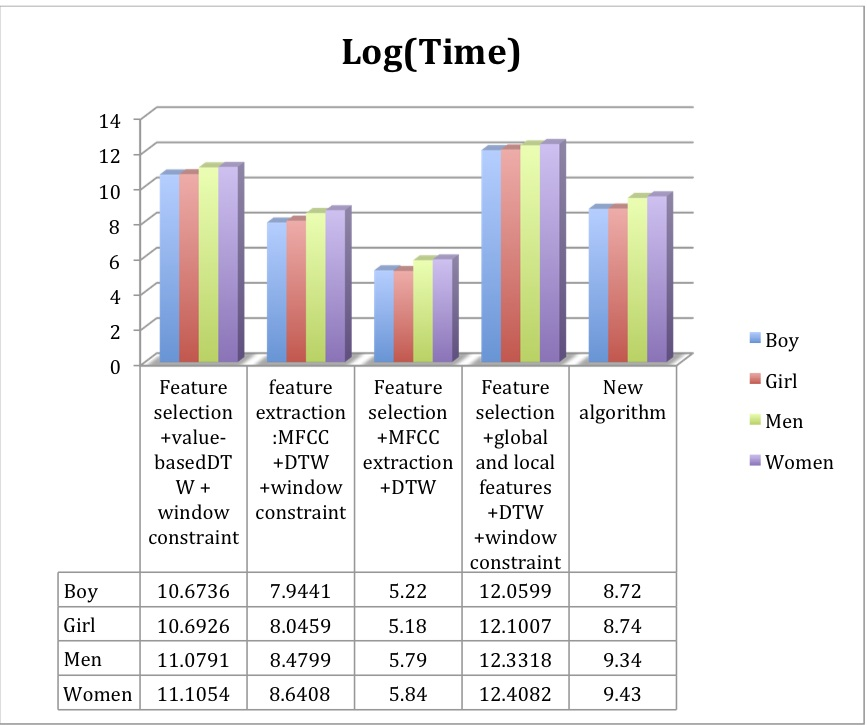
\includegraphics[scale=0.8]{GraphsResults.jpg}
  \caption{Time complexity}
  
\end{figure}
\end{spacing}

\end{document}  